\documentclass[conference]{IEEEtran}
\IEEEoverridecommandlockouts% The preceding line is only needed to identify funding in the first footnote. If that is unneeded, please comment it out.
\usepackage[utf8]{inputenc}   % soporte para acentos
\usepackage{amsmath,amssymb,amsfonts}
\usepackage{algorithmic}
\usepackage{graphicx}
\usepackage{textcomp}
\usepackage{xcolor}
\usepackage[pdftex]{hyperref}
\usepackage{hyperref}
\usepackage{algorithm}
\usepackage{float} 
\usepackage{algpseudocode}
\def\BibTeX{{\rm B\kern-.05em{\sc i\kern-.025em b}\kern-.08em
    T\kern-.1667em\lower.7ex\hbox{E}\kern-.125emX}}

\begin{document}

\title{Comparativa Quicksort}
%{\footnotesize \textsuperscript{*}Nota: Los subtítulos no son capturados en Xplore y no deben usarse}%
%\thanks{Identifique la agencia de financiación aplicable aquí. Si no hay, elimine esta línea.}}

\author{\IEEEauthorblockN{Alexis Raciel Ibarra Garnica}
\IEEEauthorblockA{\textit{Facultad de Informática} \\
\textit{Universidad Autómona de Querétaro}\\
Santiago de Querétaro, Qro, México \\
direccion.correo@email.com}
\and
\IEEEauthorblockN{Pablo Natera Bravo}
\IEEEauthorblockA{\textit{Facultad de Informática} \\
\textit{Universidad Autómona de Querétaro}\\
Santiago de Querétaro, Qro, México \\
pablonatera16@gmail.com}
}

\maketitle

\begin{abstract}
In this paper we implemented Quicksort in C sharp along with other in-place sorting algorithms such as BubbleSort, Flag BubbleSort, SelectionSort and InsertionSort.
This with the intention of comparing performance while maintaining $O(1)$ spacial complexity.
We concluded that of all the in-place sorting algorithms, Quicksort is the best option given that the pivot is chosen adequately.
\end{abstract}

\begin{IEEEkeywords}
Quicksort, Divide and Conquer, Big O.
\end{IEEEkeywords}


\section{Introducción}

El algoritmo Quicksort es uno de los algoritmos más eficientes y la 
primera elección en muchas aplicaciones debido a su flexibilidad de los distintos tipos de datos que acepta como entrada y por usar menos recursos de memoria.

\subsection{Antecedentes Históricos}
El algoritmo \textit{Quicksort}, fue desarrollado por Tony Hoare en 1959 mientras era estudiante de ciencias de la computación en la Universidad Estatal de Moscú, 
surgió de la necesidad de ordenar listas de palabras para traducirlas del ruso al inglés. 
Su propuesta superó en eficiencia al método de \textit{Insertion Sort}, haciendo uso del nuevo concepto de particiones e implementándose inicialmente en Mercury Autocode. 
Posteriormente, al regresar a Inglaterra, Hoare adaptó su idea para mejorar el algoritmo de \textit{Shellsort}, lo que lo llevó a publicar Quicksort en 1961.\cite{original_paper}
\\
Desde su primer publicación han habido diversas modificaciones con la intención de hacer aún más eficiente el algoritmo, siendo la primer de estas en 1962 por el mismo Hoare.
Otras modificaciones se basan en mejores métodos para elegir en pivote y así reducir la complejidad en el peor caso, la más popular es usando el algoritmo de Singleton.
\cite{history} 

\subsection{Divide and Conquer}
El Quicksort es un algoritmo que usa el paradigma de \textbf{Divide and Conquer}. 
Este tipo de solución implica dividir el problema en dos subproblemas independientes usando un pivote, 
cada uno siendo aproximadamente la mitad del problema original, y resolver estos subproblemas respectivamente para finalmente unir ambos en la solución final.\\
En muchas ocasiones estos subproblemas aplican de manera recursiva hasta llegar un caso base, en donde es trivial la respuesta y de ahí se van uniendo las subsoluciones hasta llegar a la solución final.
Cuando la división es balanceada, este enfoque logra reducir el número de niveles de recursión a $\log{n}$ niveles de recursión.
Otros algoritmos que ocupan este paradigma son la \textit{Búsqueda Binaria} y la \textit{Transformada Rápida de Fourier}.
\cite{divide_and_conquer}


\subsection{Algoritmo}
Aplicando el paradigma de \textit{Divide and Conquer} y el concepto de particiones se obtiene la siguiente lógica para el Quicksort\cite{Grokking}:

\begin{enumerate}
    \item Si la longitud del arreglo es menor a dos, se retorna el elemento directamente (caso base).
    \item Se selecciona un pivote (existen distintas técnicas para ello).
    \item El arreglo se reordena colocando los elementos menores al pivote a la izquierda y los mayores a la derecha. Generando así las particiones. \textbf{Divide}
    \item Los pasos anteriores se aplican recursivamente a cada partición hasta alcanzar el caso base. \textbf{Conquer}
\end{enumerate}
\\
Visto como pseudocódigo sería algo así:
\begin{algorithm}[H]
     % Sin [1] para que la línea de la función no sea numerada
    \State \textbf{Quicksort($Array, low, high$)} 
    \If {$low < high$}
        \State $pivotID \gets \Call{Partition}{Array, low, high}$
        \State \Call{Quicksort}{$Array, low, pivotID - 1$}
        \State \Call{Quicksort}{$Array, pivotID + 1, high$}
    \EndIf
\end{algorithm}

para el Quicksort. Para las particiones luciría así: 

\begin{algorithm}[H]
    \State \textbf{Partition($Array, low, high$)}
        \State $x \gets Array[high]$ 
        \State $i \gets low - 1$
        \For {$j = low$ \textbf{to} $high - 1$}
            \If {$Array[j] \leq x$}
                \State $i \gets i + 1$
                \State $\text{swap } Array[i] , Array[j]$
            \EndIf
        \EndFor
        \State $\text{swap } Array[i + 1] , Array[high]$
        \State \Return $i + 1$
\end{algorithm}

En la primera llamada \textbf{low} sería $0$ y \textbf{high} sería la longitud del arreglo menos 1.
Como se puede ver en esta implementación el pivote simplemente es el valor extremo de la derecha.

\subsection{Complejidad y pivote}
A diferencia de otros algoritmos donde la complejidad depende de la posición de los elementos en el arreglo, en Quicksort la complejidad depende casi enteramente de la elección de pivote.\cite{pivot}
\begin{enumerate}
    \item Mejor caso: se escoge un pivote que sea exactamente la mediana y cree dos particiones de la misma longitud.
Cuando esto sucede es que tenemos exactamente $\log{n}$ niveles de recursividad y cada nivel requiere $n$ operaciones, por lo que la complejidad resulta ser: $\Omega(n\cdot \log{n})$.
    \item Peor caso: si el pivote escogido genera particiones que dividen el arreglo de manera desigual ($n-1$ y $0$ elementos) en cada iteración, 
    teniendo $n$ niveles de recursividad en donde cada nivel necesita de $\approx n$ operaciones,
    resultando en una complejidad de $O(n^2)$.
    \item Paso promedio: las particiones no son perfectamente balanceadas pero ambas son siempre de longitudes mayores a cero, en este caso la complejidad también converge a $\Theta(n\cdot \log{n})$.
\end{enumerate}

Para entender mejor porque el caso promedio converge a $n \cdot\log{n}$ es útil visualizar las particiones cuando están desbalanceadas pero no de longitud cero.
En este ejemplo tenemos un arreglo en donde de manera recursiva las particiones van a tener una proporción de $1/10$ y otra de $9/10$.

\begin{figure}[h]
    \centering
    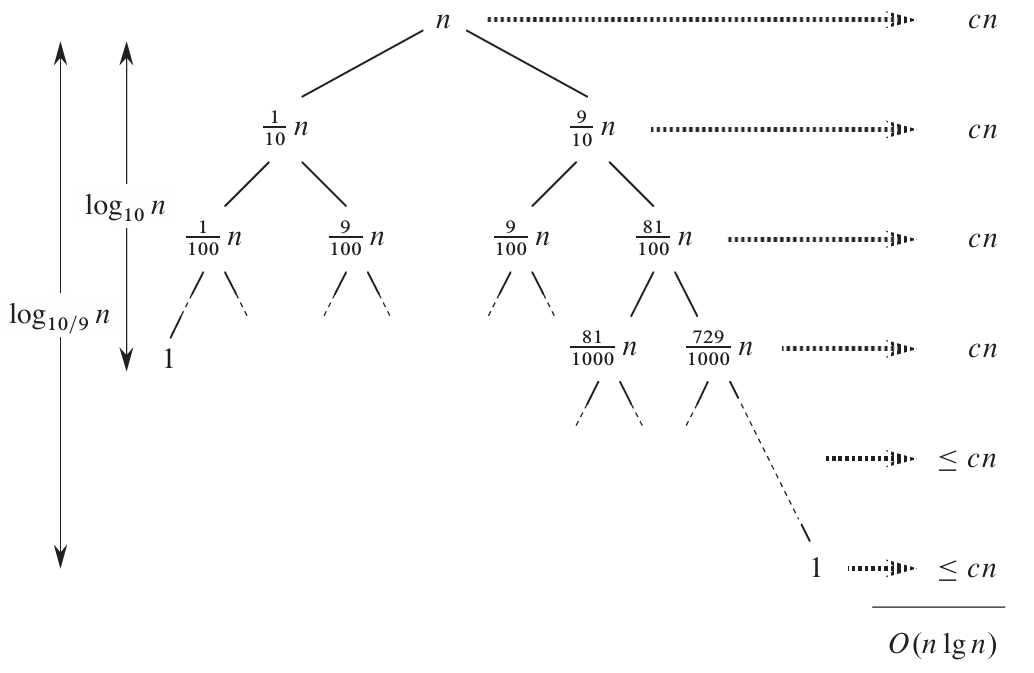
\includegraphics[scale=0.3]{convergence_avg_case.png}
    \caption{Diagrama de particiones desbalanceadas. Imagen obtenida de \cite{intro_algo}.}
    \label{fig:avg_case}
\end{figure}

En este ejemplo el número de niveles de recusrión llegará a ser $\log_{10/9}{n}$ en la rama de la derecha, y para la rama de la izquierda será $\log_{10}{n}$.
Y para cada nivel de recursión se tendrán que hacer $\approx n$ operaciones, resultando en la complejidad de: $\Theta(n\cdot \log{n})$.

Sabiendo esto es fácil entender porqué es necesaria una buena técina para escoger el pivote.
\\Una técinca muy popular y relativamente sencilla de entender el agarrar el primer, último y elemento de el medio del arreglo o partición, 
calcular su mediana y usar eso como pivote.
Esta técnica ayuda a que el quicksort pase de tener una complejidad del peor caso para arreglos ordenados al mejor caso, y también ayuda a siempre tener dos particiones de longitud distintas a cero.

\subsection{Algoritmos de ordenamiento in-place}
Quicksort es un algoritmo in-place, lo que significa que funciona haciendo intercambios sin hacer uso de estructuras de datos externas. Otros algoritmos que son in-place serían ambas versiones del Bubblesort, Insertion sort y el Selection sort.
La gran ventaja de usar este paradigma es que la complejidad espacial del algoritmo es bastante baja, $\log{n}$ en el mejor caso y caso promedio y $n$ en el peor caso.
Usando la mediana de tres para escoger el pivote también nos aseguramos de tener una complejidad espacial logarítmica.
\cite{space_complexity}

\section{Metodología}
Aquí debe describir los métodos, enfoques o procedimientos utilizados en su investigación.

\section{Resultados}
Presente los hallazgos y datos recopilados de su metodología. Incluya figuras y tablas como se muestra a continuación.


\section{Conclusiones}
El Quicksort es el mejor de los algoritmos de in-place dado que se escoga bien el pivote.


\bibliographystyle{IEEEtran}
\bibliography{biblios.bib}
\end{document}
